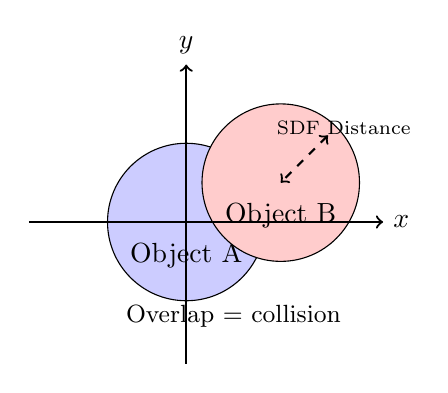
\begin{tikzpicture}
  \draw[fill=blue!20] (0,0) circle (1) node[below=4pt] {Object A};
  \draw[fill=red!20] (1.2,0.5) circle (1) node[below=4pt] {Object B};

  \draw[->, thick] (-2, 0) -- (2.5, 0) node[right] {$x$};
  \draw[->, thick] (0, -1.8) -- (0, 2) node[above] {$y$};

  \node at (0.6, -1.2) {\small Overlap = collision};
  \draw[<->, dashed, thick] (1.8,1.1) -- (1.2,0.5);
  \node at (2,1.2) {\scriptsize SDF Distance};
\end{tikzpicture}
